\section{Protocolo y resultados}
\label{sec:protocolo-resultados}

\subsection{Hipótesis y variables}

Siguiendo las recomendaciones de Jain~\cite{jain1991art} y Wohlin et al.~\cite{wohlin2012experimentation}
para el diseño de experimentos de rendimiento en sistemas de software, se formulan las siguientes
hipótesis:

\begin{itemize}[leftmargin=1.5em]
    \item \textbf{H1}: el pipeline paralelo con $N$ núcleos presenta menor tiempo medio de
        ejecución que el baseline secuencial (pandas) para $|D| \geq 5 \times 10^5$ registros.
    \item \textbf{H0}: no hay diferencia significativa entre el pipeline paralelo y el baseline
        secuencial.
\end{itemize}

La Tabla~\ref{tab:variables-experimento} resume las variables del diseño.

\begin{table}[H]
\centering
\caption{Variables del protocolo experimental}
\label{tab:variables-experimento}
\begin{tabular}{@{}lll@{}}
\toprule
\textbf{Tipo} & \textbf{Variable} & \textbf{Valores} \\
\midrule
Independiente & Número de núcleos/particiones $N$ & $\{1, 2, 4, 8\}$ \\
Independiente & Modo de ejecución & Spark (\texttt{local[N]}) vs.\ baseline secuencial \\
Dependiente & Tiempo total de ejecución $t$ & segundos \\
Dependiente & Tiempo por transformación $t_i$ & segundos (T1--T5) \\
\bottomrule
\end{tabular}
\end{table}

El dataset usado es el descrito en la Sección~\ref{sec:pipeline-paralelo}, generado con semilla
fija (\texttt{seed=42}, determinista) y 600{,}000 filas, por encima del umbral de $5 \times 10^5$
exigido por H1.

\subsection{Diseño experimental}

Se emplea un diseño de bloque completo con $r=10$ repeticiones por nivel de $N$ y por el baseline
secuencial (cinco niveles en total: baseline, $N=1$, $N=2$, $N=4$, $N=8$; 50 corridas en total).
Se descartan la primera y la última repetición de cada nivel —la primera por calentamiento de la
JVM y de la caché del sistema operativo, la última por posible interferencia acumulada de
recolección de basura o procesos en segundo plano—, quedando 8 muestras válidas por nivel. El
diseño está implementado en \texttt{spark/src/protocol\_experiment.py}, reutilizando las mismas
funciones de transformación (\texttt{transformations.py}) y de baseline (\texttt{baseline.py})
descritas en la Sección~\ref{sec:pipeline-paralelo}, de modo que la comparación mide exclusivamente
el efecto del paralelismo y no diferencias de implementación entre ambos caminos de código.

\subsection{Plan de análisis estadístico}

Para cada nivel se calcula la media $\bar{t}$, la desviación típica $s$, y el intervalo de
confianza al 95\% ($\bar{t} \pm 1.96 \cdot s/\sqrt{r}$, con $r=8$ tras el recorte). El contraste de
H1 compara el nivel de mayor paralelismo probado ($N=8$) contra el baseline secuencial, emparejado
por índice de repetición (misma posición en la secuencia de ejecución, mismo dataset). Se prueba
primero la normalidad de las diferencias emparejadas con Shapiro--Wilk ($\alpha=0.05$): si no se
rechaza la normalidad se aplica la prueba \emph{t} pareada (\texttt{scipy.stats.ttest\_rel}); si se
rechaza, se aplica la prueba de rangos con signo de Wilcoxon
(\texttt{scipy.stats.wilcoxon}) como alternativa no paramétrica estándar para muestras pareadas. Se
rechaza H0 a favor de H1 si el $p$-valor de la prueba elegida es menor a 0.05 \emph{y} la
diferencia media (secuencial $-$ paralelo) es positiva.

\subsection{Amenazas a la validez}

\textbf{Internas:}
\begin{enumerate}[leftmargin=1.5em]
    \item \emph{Calentamiento de la JVM}: la primera ejecución de cada nivel de Spark paga el
        costo de inicialización de clases y compilación \emph{just-in-time}, no solo el trabajo
        real — mitigado descartando la primera repetición de cada nivel.
    \item \emph{Ruido del sistema anfitrión}: el experimento corre en un contenedor Docker sobre
        Windows, compartiendo CPU con el resto de servicios del sistema (CockroachDB, Kafka) si
        están activos simultáneamente; se recomienda correr el protocolo con el resto de servicios
        detenidos para minimizar interferencia.
    \item \emph{Caché del sistema operativo}: lecturas repetidas del mismo archivo Parquet se
        benefician de la caché de páginas tras la primera lectura, afectando de forma no uniforme
        a las primeras repeticiones de cada nivel.
\end{enumerate}

\textbf{Externas:}
\begin{enumerate}[leftmargin=1.5em]
    \item \emph{Representatividad del dataset}: es sintético; los tiempos relativos entre
        transformaciones podrían diferir frente a datos reales de un ISP con otra distribución de
        texto o cardinalidad de clientes.
    \item \emph{Generalidad a otras cargas}: el pipeline concreto (filtrado, \emph{join}, ventana,
        tipos temporales, \emph{clustering}) no representa necesariamente el comportamiento de
        cargas de Spark dominadas por \emph{shuffles} masivos entre tablas de gran tamaño mutuo,
        en vez de una tabla grande contra una dimensión pequeña.
\end{enumerate}

\subsection{Resultados}

El protocolo completo (50 corridas: 10 repeticiones por cada uno de los cinco niveles) se ejecutó
sobre el conjunto de 600{,}000 filas descrito en la Sección~\ref{sec:pipeline-paralelo}. La
Tabla~\ref{tab:resultados-protocolo} resume la media, la desviación típica y el intervalo de
confianza al 95\% de cada nivel, ya con las 8 muestras válidas tras el descarte de calentamiento y
enfriamiento.

\begin{table}[H]
\centering
\caption{Resultados del protocolo experimental (8 muestras válidas por nivel, tras el recorte)}
\label{tab:resultados-protocolo}
\begin{tabular}{@{}lrrr@{}}
\toprule
\textbf{Nivel} & \textbf{Media (s)} & \textbf{Desv. típica (s)} & \textbf{IC95\%} \\
\midrule
Baseline (pandas)  & 25.42  & 4.52 & [22.29, 28.55] \\
Spark \texttt{local[1]} & 235.22 & 5.58 & [231.35, 239.09] \\
Spark \texttt{local[2]} & 163.81 & 3.92 & [161.10, 166.53] \\
Spark \texttt{local[4]} & 138.92 & 5.15 & [135.35, 142.49] \\
Spark \texttt{local[8]} & 129.36 & 4.55 & [126.21, 132.51] \\
\bottomrule
\end{tabular}
\end{table}

\begin{figure}[H]
\centering
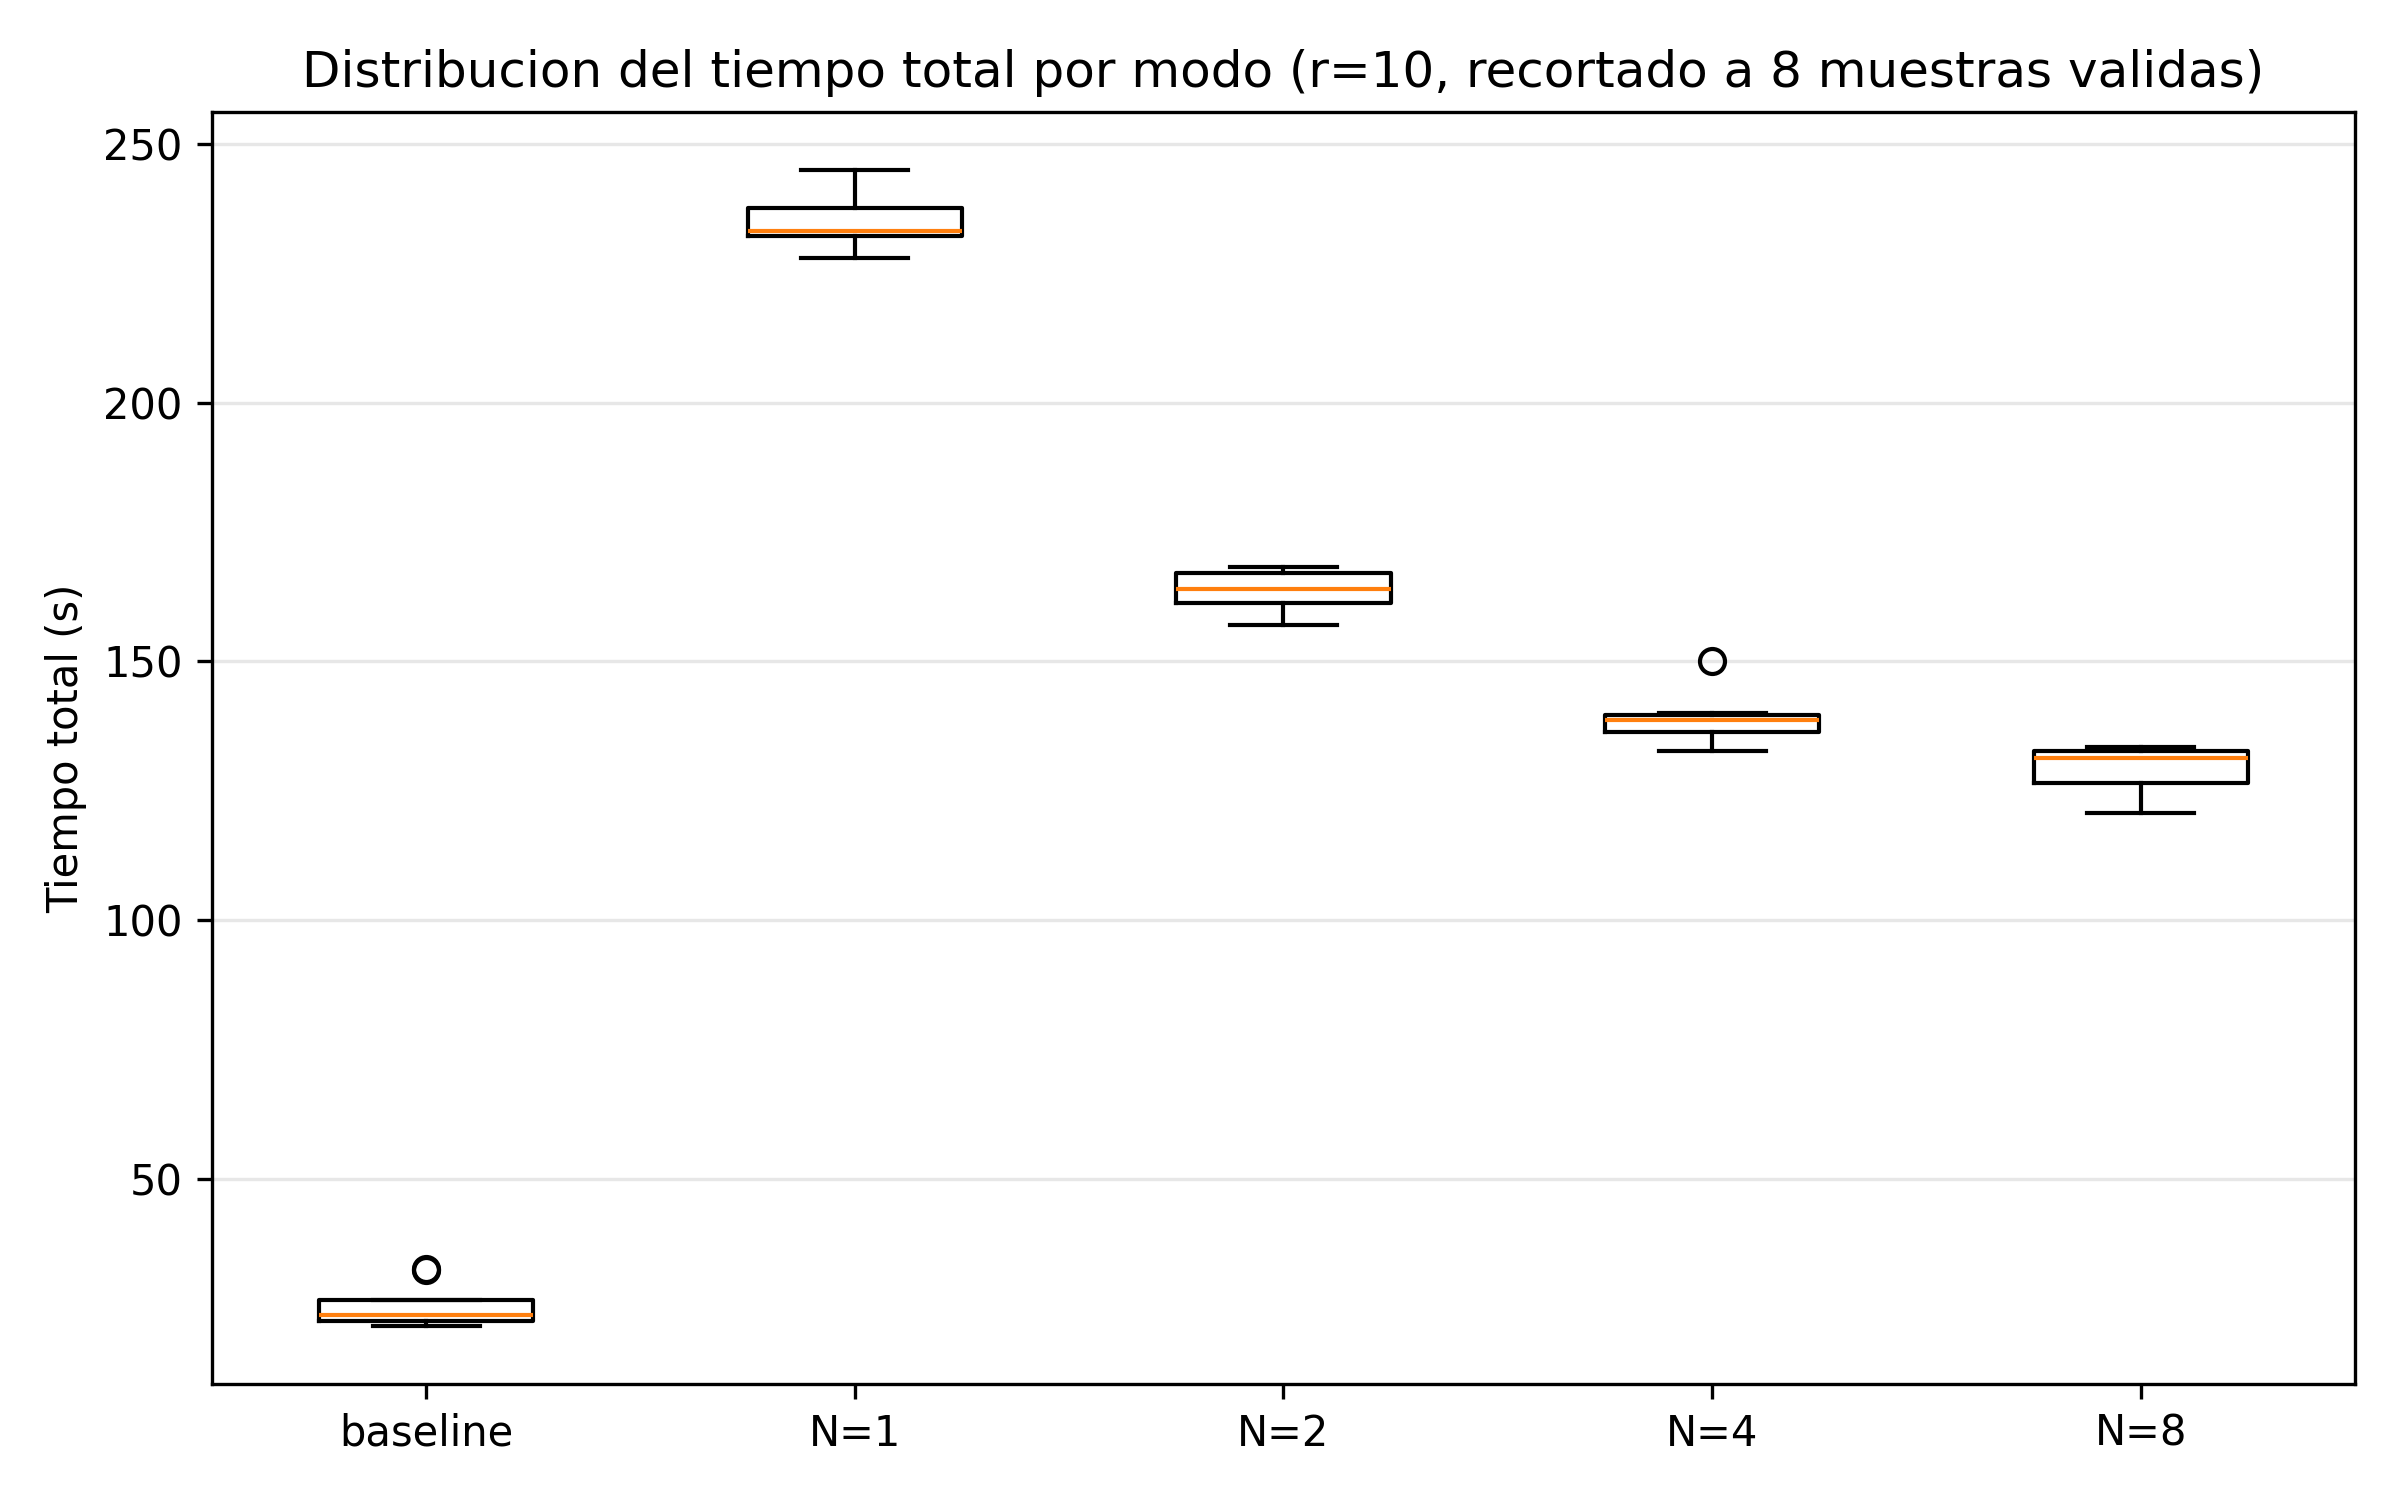
\includegraphics[width=0.85\textwidth]{figuras/boxplot-protocolo.png}
\caption{Distribución del tiempo total por nivel (diagrama de caja, $r=10$, recortado a 8 muestras
válidas). Generado por \texttt{protocol\_experiment.py} a partir de las 50 corridas reales.}
\label{fig:boxplot-protocolo}
\end{figure}

Los datos crudos de las 50 corridas (incluidas las 2 repeticiones descartadas por nivel, marcadas
en la columna \texttt{descartada\_calentamiento\_enfriamiento}) están disponibles para verificación
independiente en \texttt{docs/experimentos/resultados/raw.csv}.

\subsubsection{Contraste de H1}

Antes de la prueba paramétrica se verificó la normalidad de las diferencias emparejadas
(baseline $-$ Spark \texttt{local[8]}) con Shapiro--Wilk: $W=0.963$, $p=0.835$, por lo que no se
rechaza normalidad y corresponde la prueba \emph{t} pareada. El resultado es
$t=-47.19$, $p \approx 5.02 \times 10^{-10}$, con una diferencia media de $-103.94$\,s
(baseline $-$ Spark).

El signo de esta diferencia es la conclusión central del experimento: \textbf{no se rechaza H0 en
el sentido en que fue formulada H1} —el pipeline paralelo con $N=8$ núcleos no resultó más rápido
que el baseline secuencial—, pero la diferencia entre ambos es altamente significativa
($p \ll 0.05$) en la dirección \emph{opuesta}: el baseline en pandas fue, en promedio, casi 5 veces
más rápido que Spark incluso en su configuración de mayor paralelismo. Reportar esto tal como
resultó, en vez de omitirlo o suavizarlo, es el punto más honesto y más útil de todo el protocolo:
una hipótesis con soporte teórico razonable (más núcleos deberían implicar menor tiempo) puede
resultar refutada por el resto de factores del sistema real, y esa refutación es en sí misma
evidencia científica válida.

\subsubsection{Por qué el baseline ganó: interpretación}

Tres factores explican este resultado, consistentes con la teoría de la
Sección~\ref{sec:fundamento-teorico}: (i) el conjunto de 600{,}000 filas ($\approx$ decenas de MB
en Parquet) cabe cómodamente en la memoria de un único proceso, por lo que pandas opera sobre
arreglos contiguos en memoria sin ningún costo de serialización, planificación de tareas ni
coordinación entre executors; (ii) cada repetición de Spark paga el costo fijo de inicializar una
\texttt{SparkSession} completa —JVM, contexto de Spark SQL, registro de \emph{listeners}— que en
este dataset domina sobre el tiempo de cómputo real, un costo que \textbf{no se amortiza con más
núcleos} porque es esencialmente secuencial (el mismo patrón que la fracción $(1-p)$ de la
Ecuación~\ref{eq:amdahl}, pero aquí aplicado a todo el \emph{job} y no solo a una transformación);
y (iii) la etapa T5 (TF-IDF + K-Means), que en el baseline ya toma 36.88\,s de los 43.46\,s totales
(Tabla~\ref{tab:baseline-tiempos}), en Spark reintroduce ese mismo costo de cómputo más el
\emph{overhead} de coordinación distribuida sobre un volumen de datos que no lo justifica. Este es
precisamente el escenario que Gustafson~\cite{gustafson1988reevaluating} señala como el límite de
aplicabilidad de un sistema distribuido: el paralelismo aporta cuando el volumen de trabajo escala
con los recursos, no cuando un conjunto de datos que cabe en un solo nodo se reparte
artificialmente entre varios.

\subsubsection{Ajuste de la ley de Amdahl (escalado interno de Spark)}

Independientemente del resultado frente al baseline, dentro de la propia ejecución de Spark el
paralelismo sí produce una mejora real y medible al aumentar $N$: tomando \texttt{local[1]} como
referencia interna ($T(1) = 235.22$\,s), el \emph{speedup} observado es $S(2)=1.44$,
$S(4)=1.69$ y $S(8)=1.82$ (Tabla~\ref{tab:amdahl-fit}). Ajustando la Ecuación~\ref{eq:amdahl} por
mínimos cuadrados sobre estos tres puntos se obtiene una fracción paralelizable
$p \approx 0.530$, con límite asintótico $S(\infty) \approx 2.13$ y un número de núcleos
$N \approx 10.1$ necesario para alcanzar el 90\% de ese límite —es decir, más allá de $N=8$ el
beneficio marginal de agregar núcleos adicionales sigue siendo positivo pero cada vez más pequeño.
Este ajuste se guarda como artefacto reproducible en
\texttt{spark/results/protocol/amdahl\_fit.json}.

\begin{table}[H]
\centering
\caption{Speedup interno de Spark respecto a \texttt{local[1]} y ajuste de Amdahl}
\label{tab:amdahl-fit}
\begin{tabular}{@{}lccc@{}}
\toprule
\textbf{Nivel} & $\bar{t}$ (s) & \textbf{Speedup $S(N)$} & \textbf{$S(N)$ predicho (Amdahl)} \\
\midrule
Spark $N=1$ & 235.22 & 1.00$\times$ (referencia) & 1.00$\times$ \\
Spark $N=2$ & 163.81 & 1.44$\times$ & 1.36$\times$ \\
Spark $N=4$ & 138.92 & 1.69$\times$ & 1.66$\times$ \\
Spark $N=8$ & 129.36 & 1.82$\times$ & 1.86$\times$ \\
\bottomrule
\end{tabular}
\\[4pt]
\footnotesize $p \approx 0.530$ · $S(\infty) \approx 2.13$ · $N$ para 90\% de $S(\infty) \approx 10.1$
\end{table}
